\subsection{Instalación de JMeter (Ubuntu)}

Antes de instalar JMeter tenemos que instalar docker y docker-compose para poder descargar el repositorio que se proporciona:

\begin{lstlisting}[language=bash]
    sudo apt-get install docker docker-compose
\end{lstlisting}

Ahora vamos a descargar el repositorio de JMeter proporcionado para hacer la práctica con el siguiente comando:

\begin{figure}[H]
    \centering
    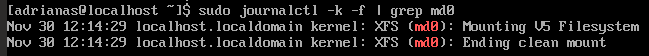
\includegraphics[scale=0.45]{JMeter/img2}
    \caption{Descarga de la carpeta con JMeter}
\end{figure}

Una vez descargada la carpeta, iniciamos el servicio con el comando:

\begin{lstlisting}[language=bash]
    sudo docker-compose up
    sudo docker-compose down
\end{lstlisting}

up para levanatar el servicio y down para pararlo. La ejecución de docker ensucia mucho la pantalla con muchos outputs. Para que no 
que no imprima nada por pantalla, ejecutamos el siguiente comando:

\begin{figure}[H]
    \centering
    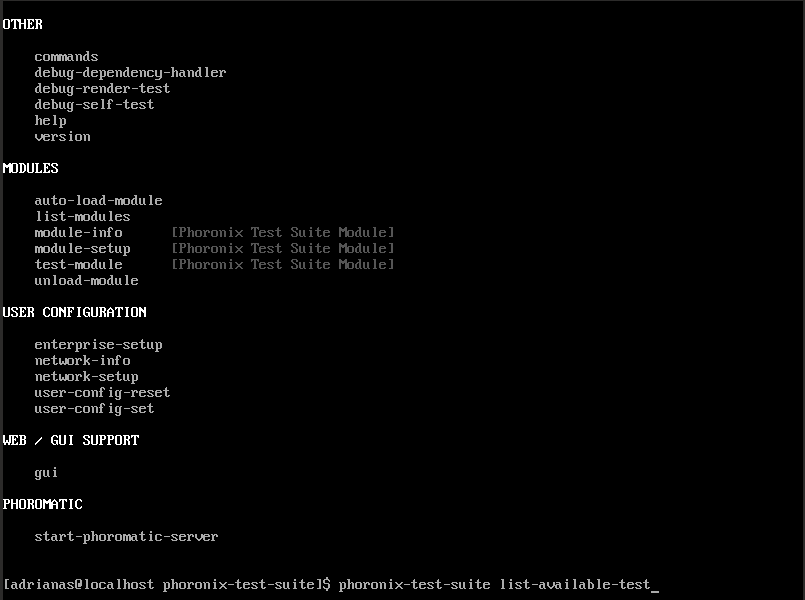
\includegraphics[scale=0.5]{JMeter/img7}
    \caption{Levantar el servicio sin outputs}
\end{figure}

La primera vez tardará un rato ya que tendrá que descargar todos los contenedores. Una vez termine, tendremos que habilitar el puerto 3000 ya que el servicio lo requiere.
Esto, como ya sabemos, lo haremos con el comando:

\begin{lstlisting}[language=bash]
    ufw enable
    ufw allow 3000/tcp    
\end{lstlisting}

Para ver si todo se ha iniciado correctamente, lo comprobamos en un navegador poniendo la IP de nuestro servidor seguido del puerto 3000 y tendría que salir un resultado como el siguiente:

\begin{figure}[H]
    \centering
    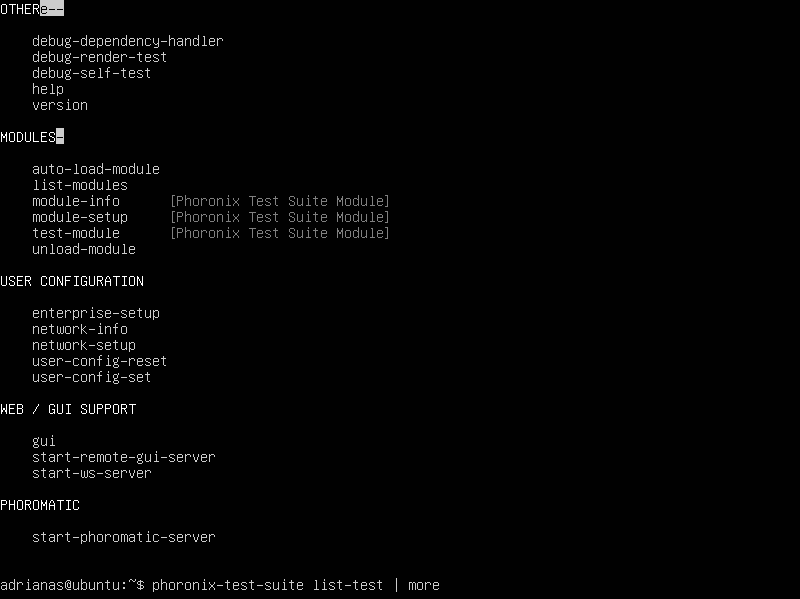
\includegraphics[scale=0.4]{JMeter/img6}
    \caption{Pantalla de inicio del servicio}
\end{figure}

\subsection{Instalación de JMeter en nuestro Host}

El único requisito que tiene JMeter para permitir su ejecución es tener Java instalado y lo podemos comprobar con la ejecución del comando:

\begin{lstlisting}[language=bash]
    java --version
\end{lstlisting}

Una vez comprobamos que tenemos Java instalado, nos vamos a la página oficial de JMeter y lo descargamos. Al descomprimirlo nos vamos a su carpeta y ejecutamos el archivo cuyo nombre es ApacheJMeter.jar:

\begin{figure}[H]
    \centering
    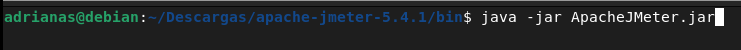
\includegraphics[scale=0.5]{JMeter/img11}
    \caption{Ejecución con Java de JMeter.}
\end{figure}

Al abrirlo nos aparecerá una ventana como la siguiente:

\begin{figure}[H]
    \centering
    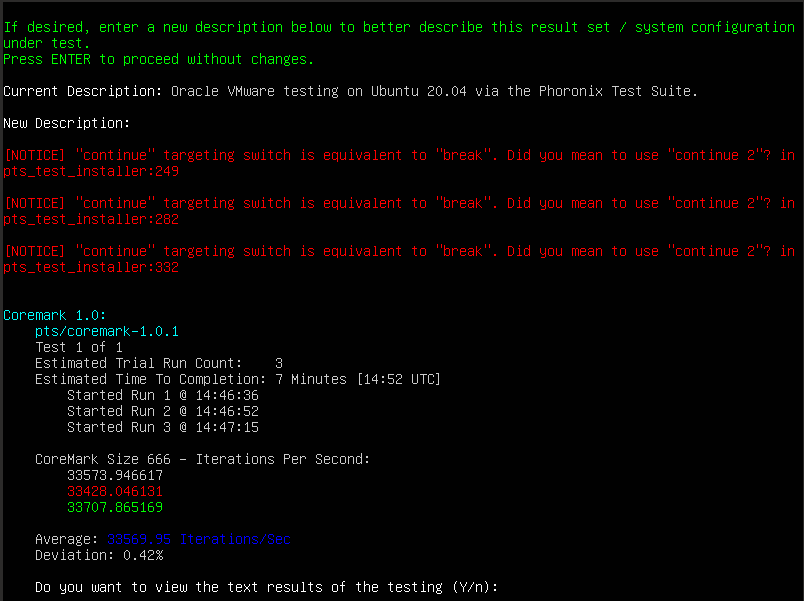
\includegraphics[scale=0.25]{JMeter/img12}
    \caption{Pantalla inicial de JMeter}
\end{figure}

\subsubsection{Parametrizar el Host y el Puerto en el Test Plan}

Para lograr parametrizar el Host y el Puerto tenemos que añadir al nodo principal los datos de nuestra IP y el Puerto:

\begin{figure}[H]
    \centering
    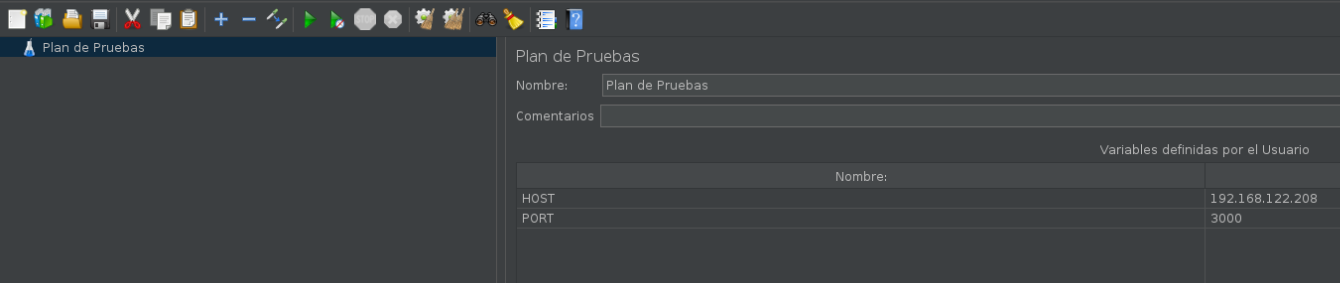
\includegraphics[scale=0.3]{JMeter/img13}
    \caption{Añadimos las variables de HOST y PORT}
\end{figure}

\newpage
\subsubsection{Hacer dos grupos de hebras distintos para alumnos y administradores para simular el acceso concurrente}

Para ello lo primero que tenemos que hacer es ver los archivos .csv que se encuentran en la carpeta iseP4JMeter/jMeter. Ahí encontraremos los archivos alumnos.csv y administradores.csv. Miramos su contenido y cogemos una cuenta de cada uno de los archivos:

\begin{figure}[H]
    \centering
    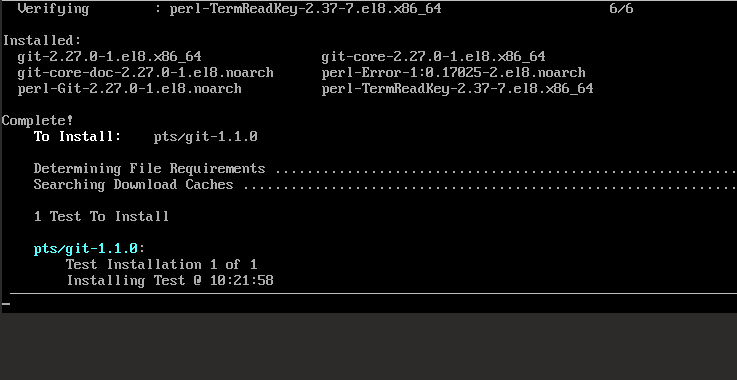
\includegraphics[scale=0.5]{JMeter/img15}
    \caption{Archivo administradores.csv}
\end{figure}

\begin{figure}[H]
    \centering
    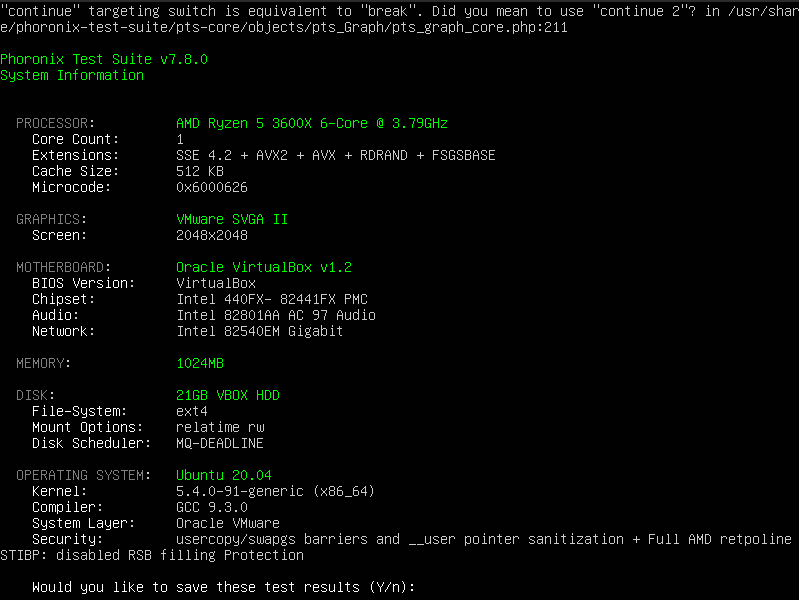
\includegraphics[scale=0.3]{JMeter/img17}
    \caption{Archivo alumnos.csv}
\end{figure}

Una vez tenemos ambas cuentas, vamos a JMeter y añadimos dos grupos de hebras que simularán el acceso de los administradores y de los alumnos.

\begin{figure}[H]
    \centering
    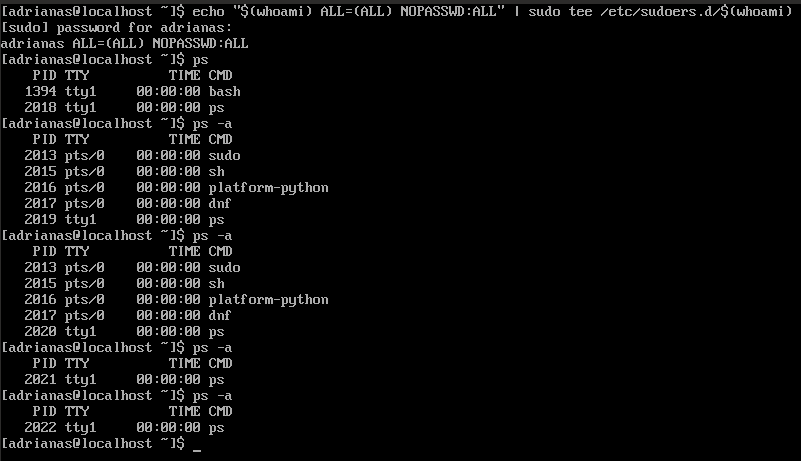
\includegraphics[scale=0.3]{JMeter/img19}
    \caption{Añadimos dos grupos de hebras}
\end{figure}

Yo he dejado todo por defecto en cada uno de los grupos de hebras. Añadimos un elemento de configuración HTTP por defecto para que en las peticiones que añadiremos a continuación tengan la IP y el Puerto configurados por defecto.

\begin{figure}[H]
    \centering
    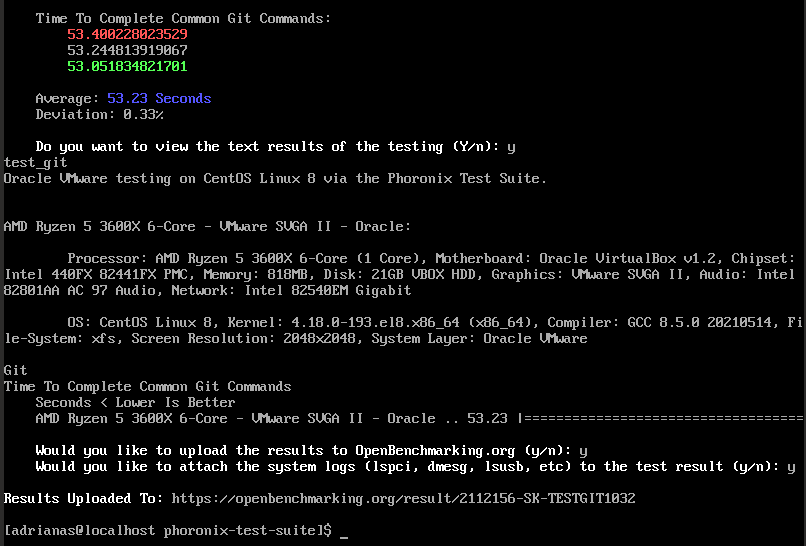
\includegraphics[scale=0.25]{JMeter/img21}
    \caption{Valores por defecto para las Peticiones HTTP}
\end{figure}

En la imagen añado un elemento a cada hebra, aunque lo más adecuado es añadirlo en general al plan de pruebas (lo hago más adelante).

Lo siguiente que tenemos que hacer es añadir una petición HTTP a cada una de las hebras para simular un login de un administrador y de un alumno:

\begin{figure}[H]
    \centering
    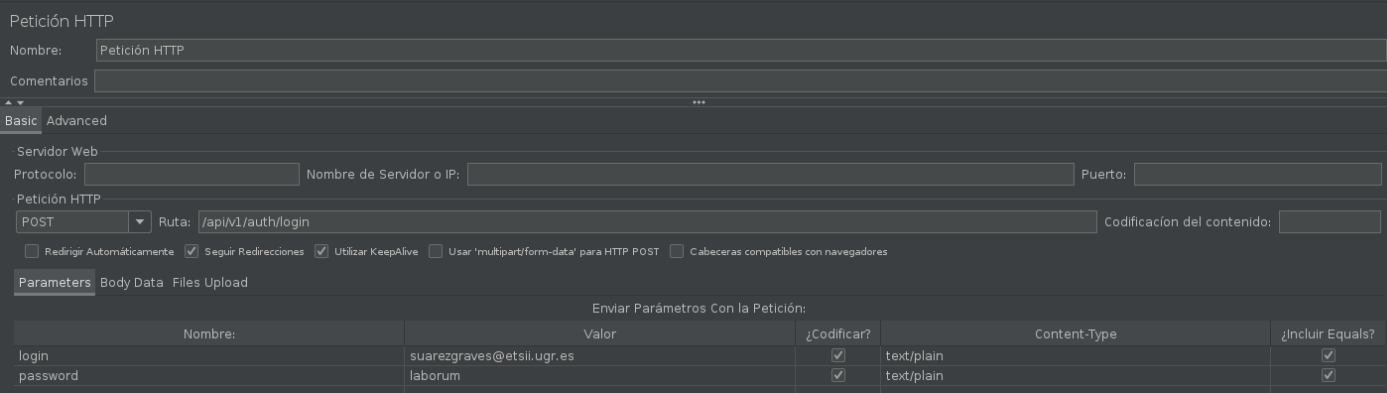
\includegraphics[scale=0.3]{JMeter/img22}
    \caption{Login de administrador}
\end{figure}

\begin{figure}[H]
    \centering
    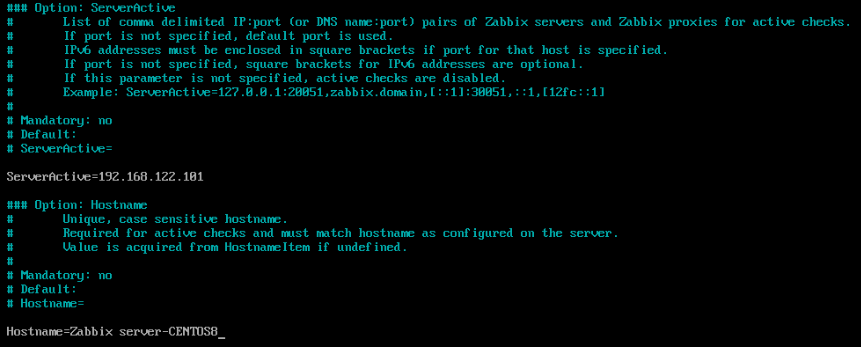
\includegraphics[scale=0.3]{JMeter/img23}
    \caption{Login de usuario}
\end{figure}

Para poder ver los resultados de ambas peticiones añadimos un árbol de resultados por defecto y ejectuamos el plan de pruebas:

\begin{figure}[H]
    \centering
    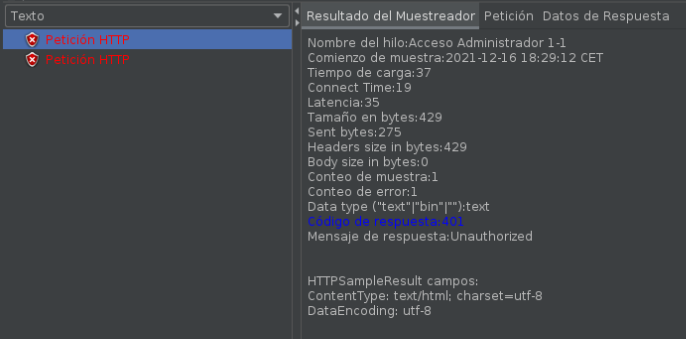
\includegraphics[scale=0.5]{JMeter/img25}
    \caption{Ejecución del plan de pruebas}
\end{figure}

Como vemos nos da error en ambos login. Esto es porque no tenemos autorización. El acceso está protegido con un BasicAuth donde el usuario es etsiiApi y la contraseña laApiDeLaETSIIDaLache. Esto aparece en la página de inicio que vimos antes.
Para solucionar este error añadimos en cada uno un gestor de autorización  HTTP con los datos ya mencionados:

\begin{figure}[H]
    \centering
    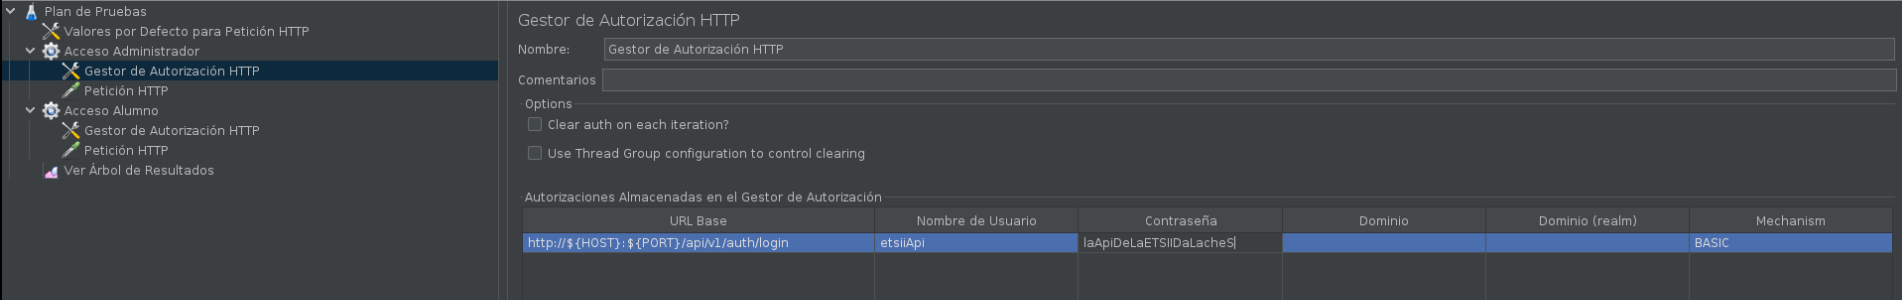
\includegraphics[scale=0.25]{JMeter/img27}
    \caption{Configuración del gestor de Autorización HTTP}
\end{figure}

\begin{figure}[H]
    \centering
    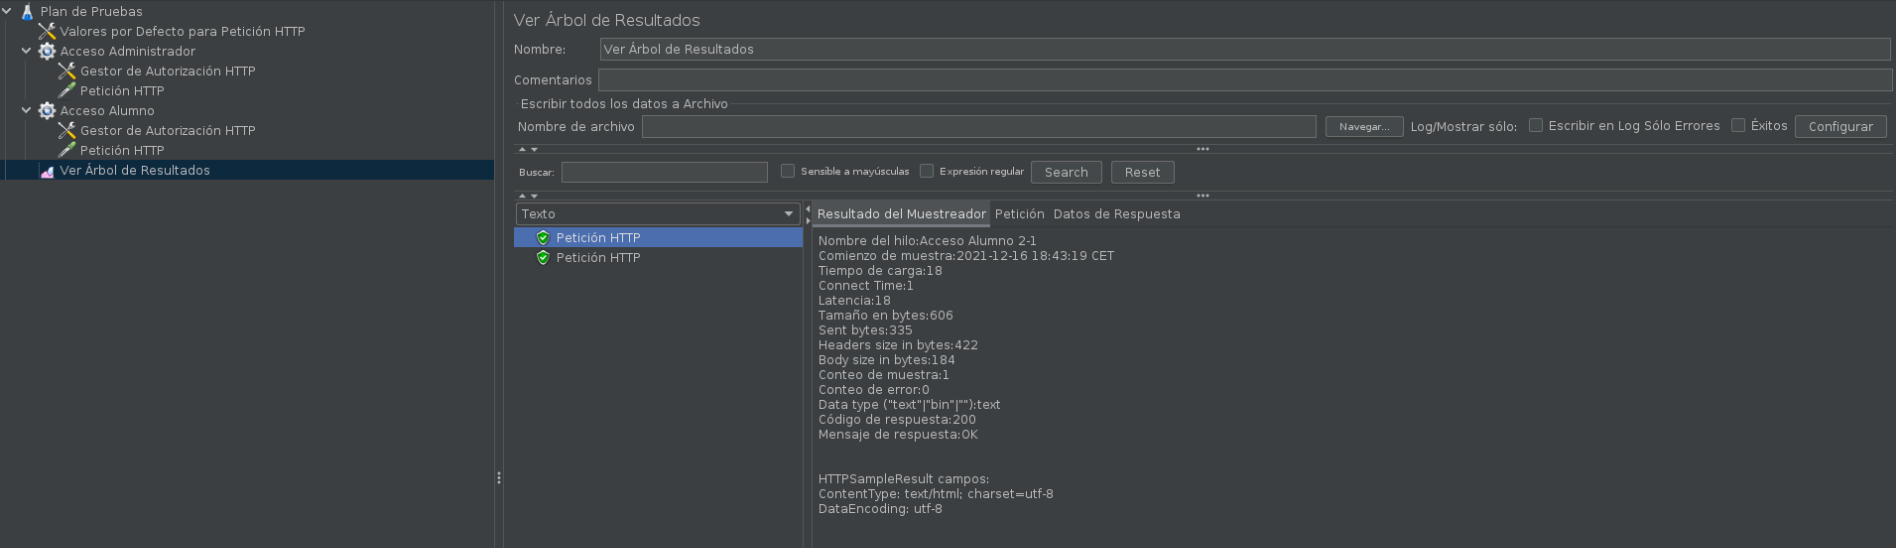
\includegraphics[scale=0.25]{JMeter/img28}
    \caption{Resultados correctos de los login}
\end{figure}

\subsubsection{Extracción del token JWT con expresiones regulares}

Para poder guardar el token que nos devuelven ambos login tenemos que crear un extractor de expresiones regulares como aparece en la siguiente imagen:

\begin{figure}[H]
    \centering
    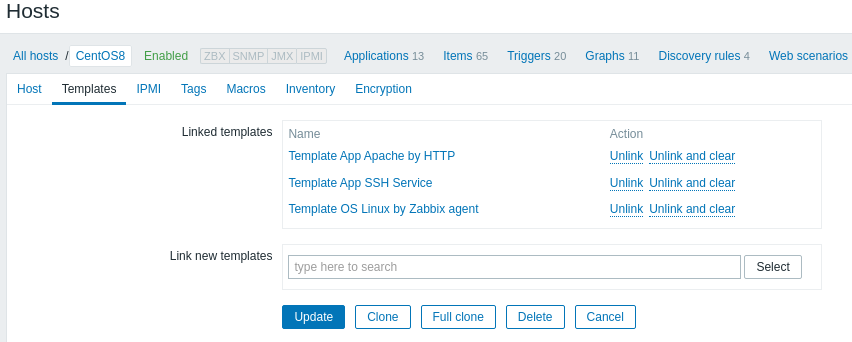
\includegraphics[scale=0.3]{JMeter/img29}
    \caption{Extractor de expresiones regulares}
\end{figure}

Para poder recibir la información usando un GET y el token hace falta que creemos otra petición HTTP donde pondremos solo la ruta del correo del alumno que queremos mostrar:

\begin{figure}[H]
    \centering
    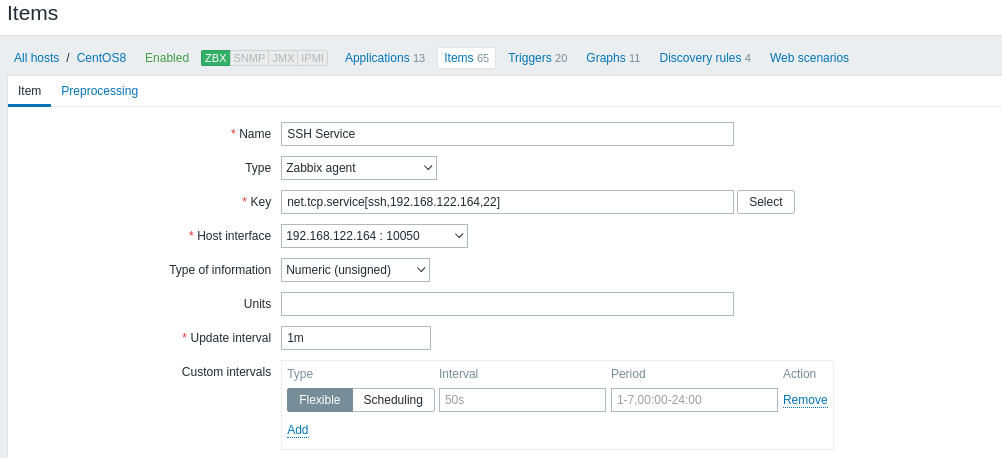
\includegraphics[scale=0.25]{JMeter/img31}
    \caption{Petición HTTP GET}
\end{figure}

También tenemos que indicar el método de seguridad usando el token que se ha recibido. Esto se hace con un gestor de cabecera HTTP, el cual se lo pondremos a la petición HTTP GET del administrador.

\begin{figure}[H]
    \centering
    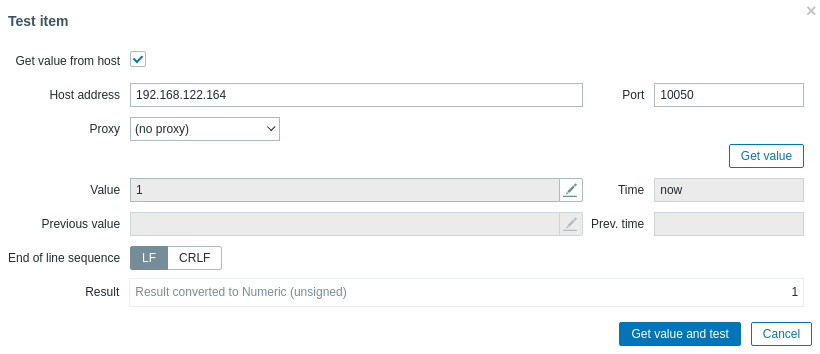
\includegraphics[scale=0.3]{JMeter/img32}
    \caption{Gestor de cabecera HTTP}
\end{figure}

Y podemos ver que funciona correctamente:

\begin{figure}[H]
    \centering
    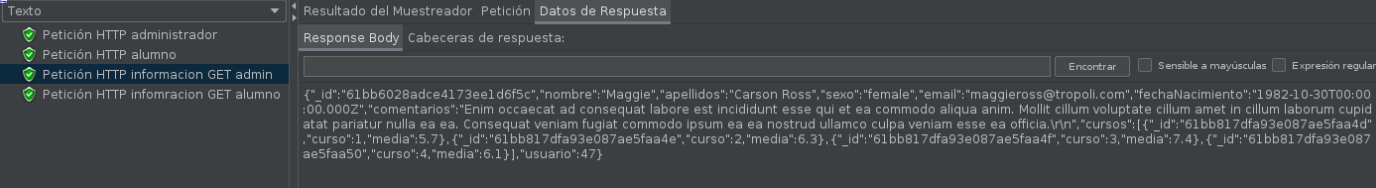
\includegraphics[scale=0.3]{JMeter/img33}
    \caption{Ejecución del plan de pruebas para comprobar si funciona}
\end{figure}

Pero para comprobar que funcione correctamente, si le indicamos un correo de un alumno en vez de un administrador pasa lo siguiente:

\begin{figure}[H]
    \centering
    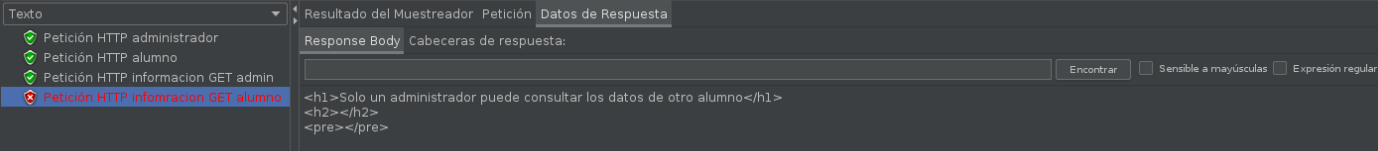
\includegraphics[scale=0.3]{JMeter/img34}
    \caption{Cambio de correo por el de un alumno}
\end{figure}

\subsubsection{Esperas aleatorias a cada grupo de hebras}

Con el objetivo de simular un entorno más realista, le añadimos a cada uno de los grupos de hebras un temporizador aleatorio Gaussiano como se ve en la siguiente imagen:

\begin{figure}[H]
    \centering
    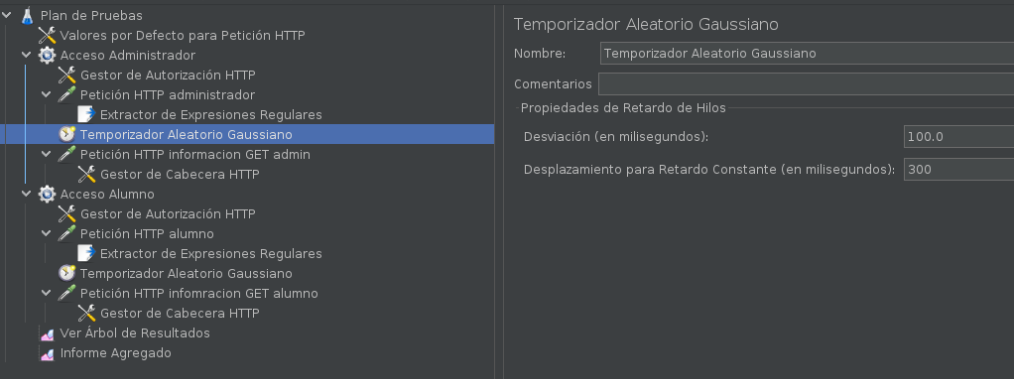
\includegraphics[scale=0.3]{JMeter/img36}
    \caption{Adición de temporizador aleatorio Gaussiano}
\end{figure}

\newpage
\subsubsection{Peticiones HTTP de los login de Alumno y Administrador}

Para ello lo primero que tenemos que hacer es añadir un elemento llamado CSV Data Set donde se accederá a los usuarios.

En la imagen hay un fallo y es que el archivo no se accede desde donde pongo. Tuve que descargar el repostorio en el host y buscar el archivo manualmente.
\begin{figure}[H]
    \centering
    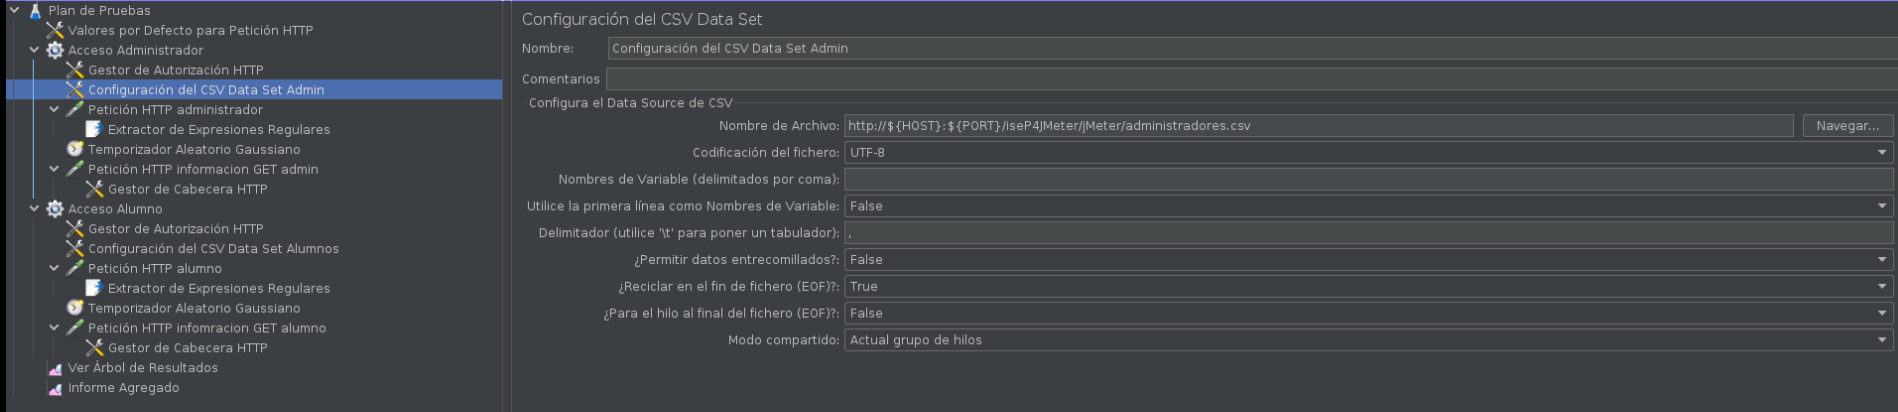
\includegraphics[scale=0.25]{JMeter/img37}
    \caption{Configuración del CSV Data Set}
\end{figure}

Y lo mismo para los alumnos. Luego hacemos una petición HTTP GET donde pondremos la siguiente información de login:

\begin{figure}[H]
    \centering
    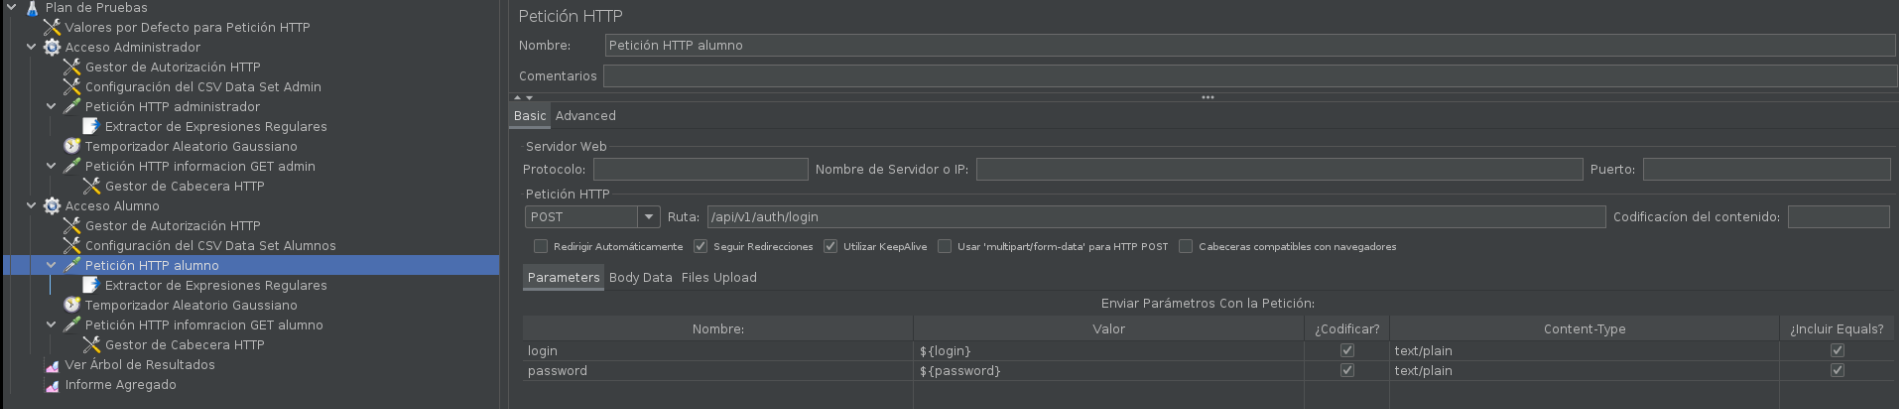
\includegraphics[scale=0.25]{JMeter/img39}
    \caption{Login de alumnos}
\end{figure}

Y al probar el plan de tests:

\begin{figure}[H]
    \centering
    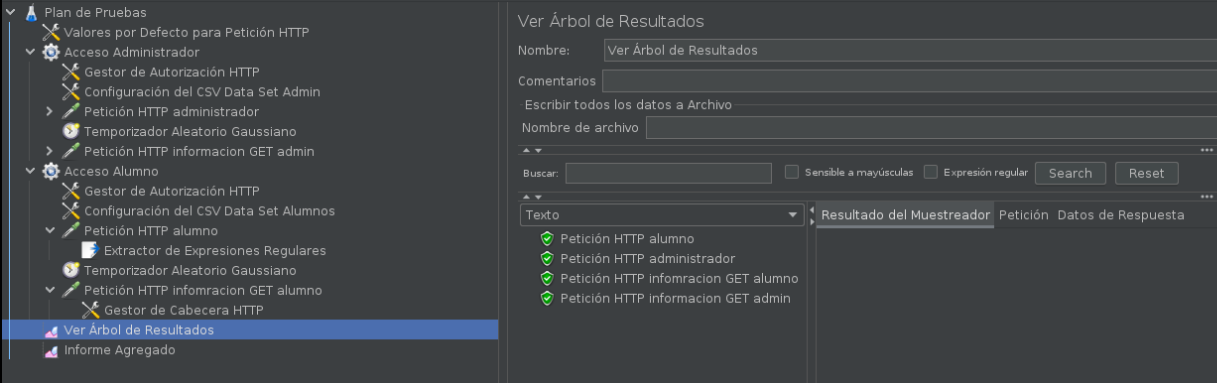
\includegraphics[scale=0.3]{JMeter/img40}
    \caption{Prueba de logins}
\end{figure}

\subsubsection{Muestreo para simular el acceso de administradores}
Lo primero que tenemos que hacer es deshabilitar la petición GET del adminsitrador.

\begin{figure}[H]
    \centering
    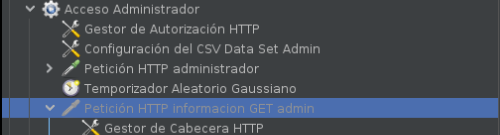
\includegraphics[scale=0.5]{JMeter/img43}
    \caption{Deshabilitamos la peticion GET del administrador}
\end{figure}

Luego tenemos que añadir un muestreador de Acceso a Log:

\begin{figure}[H]
    \centering
    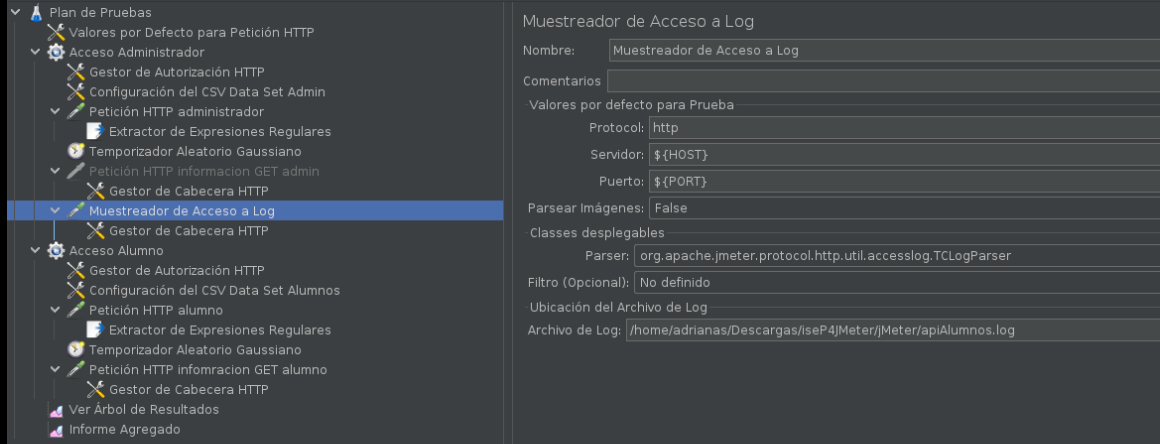
\includegraphics[scale=0.3]{JMeter/img44}
    \caption{Muestreador de Acceso a Log}
\end{figure}

Y por últmo añadimos la cabecera donde le pasamos el token de la sesión de administrador y con esto acabaríamos la práctica.
El resultado sería el siguiente:

\begin{figure}[H]
    \centering
    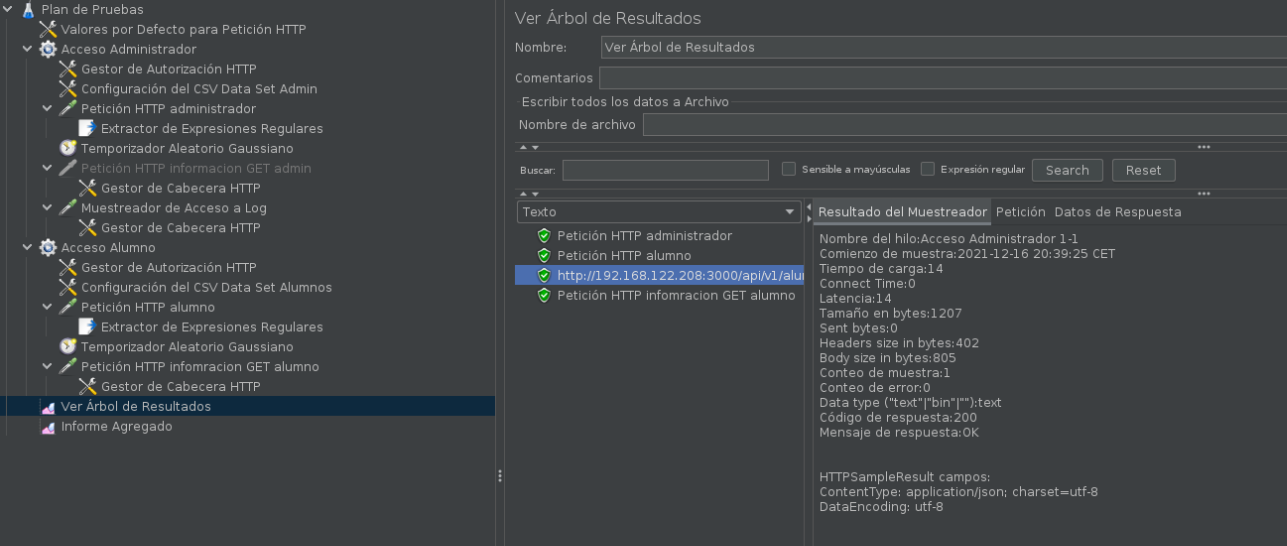
\includegraphics[scale=0.3]{JMeter/img45}
    \caption{Árbol de resultados final}
\end{figure}